\section{Examples} % (fold)
\label{sec:Examples}This section shows some examples implemented with the
Sequence Library. This is to show the variable usage of the Sequence Library.
In the beginning, the examples are relatively easy to understand. In the course
of the section, the examples become more sophisticated.

\subsection{Fibonacci Sequence}
\label{sub:Fibonacci Sequence}
Listing~\ref{lst:fibonacci_sequence} shows the implementation of the Fibonacci Sequence.

\begin{lstlisting}[
  style=ES6, 
  caption=Fibonacci Sequence,
  label={lst:fibonacci_sequence}
  ]
const FibonacciSequence = () => {

  const fibonacciIterator = () => {
    let last = 0;
    let secondLast = 0;

    const next = () => {*'\label{line:start_next}'*
      let current = last + secondLast;*'\label{line:fibonacci_calc}'*
      if (current === 0) current = 1;
      secondLast = last;
      last = current;
      return { done: false, value: current };
    };*'\label{line:end_next}'*


    return { next };
  };

  return createMonadicSequence(fibonacciIterator);
};
\end{lstlisting}
Line~\ref{line:start_next} to \ref{line:end_next} shows the |next| function. |next| is responsible for calculating an
element based on the previous. As we see on line~\ref{line:fibonacci_calc}, the current element is the
sum of the last and the second last, which represents the Fibonacci sequence.

\subsection{Fizz Buzz}
\label{sub:Fizz Buzz}
FizzBuzz is a children's game that also serves as a programming task. Frege
Goodness~\cite{frege_goodness} includes a detailed description of the game.
It is about adding rules to a sequence of numbers, where if there is a multiple
of a number, the number is replaced by a word. Listing 3 shows a part of the
implementation with the Sequence Library.

\begin{lstlisting}[
  style=ES6, 
  caption=Fizz Buzz,
  label={lst:fizz_buzz}
  ]
import * as _ from "./src/sequence/sequence.js";

const infiniteNumbers = _.Sequence(1, _ => true, i => i + 1);

const createSequenceForRule = rule =>
  _.pipe(
    // add rule's text to number
    _.map(a => a === rule.getNr() ? rule.getText() : ""),     
    _.take(rule.getNr()), // abort on this rules number
    _.cycle
  )(infiniteNumbers);

const buildFizzBuzz = () => {
  const currentRules = model.rulesSnapshot().map(createSequenceForRule);

  const baseLine  = _.Sequence("", _ => true, _ => "");
  const fizzBuzz  = _.pipe(
      // reduce to single sequence by combining all iterable values
    _.reduce$((acc, cur) =>       
    _.zipWith((a, b) => a + b)(acc)(cur), // combine all strings
    baseLine),  // start value (empty strings)

    _.zipWith((numbers, pattern) => pattern === "" 
                                     ? String(numbers) 
                                       // add numbers where no text is present
                                     : pattern
                                     )(infiniteNumbers), 
    // limit output
    _.take(model.getUpperBoundary()),
    _.drop(model.getLowerBoundary() -1),
  )(currentRules);

  model.setResult(fizzBuzz);
};
\end{lstlisting}
Listing~\ref{lst:fizz_buzz} shows two functions, |createSequenceForRule|, and
|buildFizzBuzz|. 
The |createSequenceForRule| function is called with an argument |rule| representing a
|Number| and a |String|. The returned infinite sequence then contains the
corresponding text at each multiple of the |rule|s |Number|. In the remaining places, it
contains an empty |String|. The function |buildFizzBuzz| reduces all sequences
representing a rule to a single sequence. As a demonstration,
Figure~\ref{fig:fizzbuzz_control} and \ref{fig:fizzbuzz_result} shows a
screenshot of a simple application, which shows two rules and the resulting
sequence. The tool demonstrates the possibility adding new rules at runtime. 


\begin{figure}
\centering
\begin{minipage}{.5\textwidth}
  \centering
  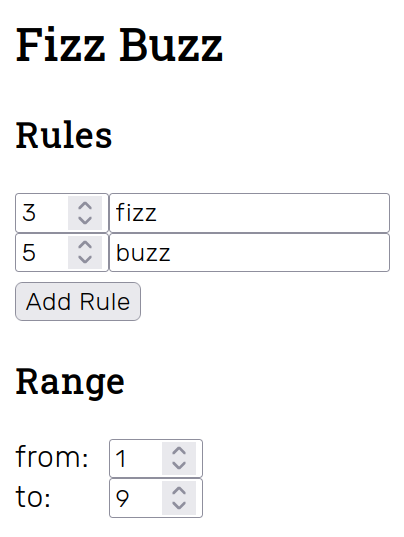
\includegraphics[width=.6\linewidth]{./mainmatter/pictures/fizzbuzz_control.png}
  \captionof{figure}{Fizz Buzz controls}
  \label{fig:fizzbuzz_control}
\end{minipage}%
\begin{minipage}{.5\textwidth}
  \centering
  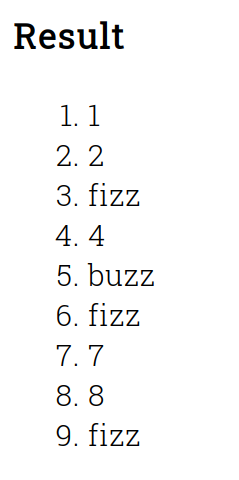
\includegraphics[width=.4\linewidth]{./mainmatter/pictures/fizzbuzz_result.png}
  \captionof{figure}{Fizz Buzz result}
  \label{fig:fizzbuzz_result}
\end{minipage}
\end{figure}


\subsection{JINQ}
\label{JINQ}
The following examples use |JINQ| to process a JSON files.

\subsubsection{Find all Students}
\label{subsub:Find all Students}
Therefore, we want to filter out all participants that have
a student ID. As you can see in the excerpt of the JSON file, this property is
not defined for all persons. Because the |JsonMonad| works in the background with
|MaybeType|, such situations can be processed without null handling.

\begin{lstlisting}[
  style=json, 
  caption=Exerpt of a JSON File including developers,
  label={lst:json_file_devs}
  ]
[
  {
    "id": 1,
    "name": "",
    "age": 28,
    "salary": 50000,
    "favoriteLanguages": [1, 3, 5]
  },
  {
    "id": 2,
    "switch-edu-id": "12-432-23",
    "name": "Emma Johnson",
    "age": null,
    "salary": 60000,
    "favoriteLanguages": [2, 4]
  },
  {
    "id": 3,
    "name": "Sophia Davis",
    "age": 40,
    "salary": null,
    "favoriteLanguages": [null, 4, 5]
  },
  ...
 ]
\end{lstlisting}


\begin{lstlisting}[
  style=ES6, 
  caption=JINQ Example - find all students,
  label={lst:jinq_find_students}
  ]
const findAllStudentIds = developers => {
  const allIds =
    from(JsonMonad(developers))
      .select(x => x['switch-edu-id'])
      .result();
};
\end{lstlisting}

\subsubsection{Find Sophia's Programming Languages}
\label{subsub:Find Sophia's Programming Languages}

This example combines two JSON files. We use the JSON file from the previous
example and the one from Listing~\ref{lst:json_file_lang}.
Listing~\ref{lst:jinq_sophias_langs} shows the code that selects Sophia's favorite programming languages from two JSON files.

\begin{lstlisting}[
  style=json, 
  caption=Exerpt of a JSON File including programming languages,
  label={lst:json_file_lang}
  ]
[
  {
    "id": 1,
    "name": "Java"
  },
  ...
  {
    "id": 4,
    "name": "C++"
  },
  {
    "id": 5,
    "name": "Haskell"
  }
]
\end{lstlisting}

\begin{lstlisting}[
  style=ES6, 
  caption=JINQ example - find Sophia's programming languages,
  label={lst:jinq_sophias_langs}
  ]
const sophiasProgrammingLanguages = (devs, languages) =>
    from(JsonMonad(devs))
      .where   ( dev    => dev.name === "Sophia Davis")
      .select  ( sophia => sophia.favoriteLanguages)
      .pairWith( JsonMonad(languages) )
      .where   ( ([langId, language]) => langId === language.id )
      .select  ( ([     _, language]) => language.name )
      .result  ();
\end{lstlisting}

\subsection{Differentiation}
\label{sub:Differentiation}
This example shows a mathematical use case, the differentiation using sequences.

\begin{lstlisting}[
  style=ES6, 
  caption=Differentiation using Sequences,
  label={lst:diff_sequences}
  ]
const halve   = x => x / 2;
const repeatF = (f, x) => _.Sequence(x, _ => true, f);

const halves = h0 => repeatF( halve, h0);


const slope = f => x => h => (f(x + h) - f(x)) / h;

const differentiate = h0 => f => x => _.map ( slope(f)(x) ) (halves(h0));
\end{lstlisting}

Listing~\ref{lst:diff_sequences} implements the following steps: 


\begin{itemize}
  \item{|repeatF| repeatedly applies the function $f$ to a value of the
    previous calculated result, starting with $x$.}
  \item{ |halves| is using |repeatF| and |halve| to halve a value $h0$. With
      that, the value $h0$ is halved again and again.} 
    \item{|slope| calculates the slope of a function $f$ at the position $x$
      with delta $h$.}
 \end{itemize}

We already have everything needed to be able to differentiate.  The function
differentiate calculates at a given point $x$ the slope more and more exactly.
Since this is an infinite sequence, we have to define one more function.
Listing~\ref{lst:impl_within} shows the function |within|, which allows differentiating until a
given epsilon.

\begin{lstlisting}[
  style=ES6, 
  caption=Implementation of within,
  label={lst:impl_within}
  ]
const parabola = x => x * x;

const diffs = differentiate(0.5)(parabola)(1); *'\label{line:diffs}'*

const within = eps => sequence => {
  const [a, rest] = _.uncons(sequence);
  const [b]       = _.uncons(rest);
  const diff      = Math.abs(a - b);

  if (diff <= eps) return b;
  return within(eps)(rest);
};
const slopeOfFAtX = within(0.000_1)(diffs);
\end{lstlisting}

Listing~\ref{lst:impl_within} defines the following implementations:

\begin{itemize}
  \item{|parabola| is the function to work with in this example}
  \item{On line~\ref{line:diffs}, |diffs| defines a function to differentiate the |parabola| at point $1$ with
    starting value $h0$ of $0.5$.}
  \item{|within| calculates recursively the slope of the |parabola| using the
      sequence |diffs| until a satisfying accuracy. 
    \item{ At the end, |slopeOfFAtX| calculates the slope with the given parameters. }
    }
\end{itemize}


\subsection{Alpha - Beta Algorithms}
\label{Alpha - Beta Algorithms}

